\FloatBarrier{}
\section{Estado de la cuestión}%
\label{sec:state}

\begin{revisado}

Se realizó un relevamiento de la literatura existente que cubre el procesamiento de correos electrónicos tanto de
reservas de tickets aéreos como de estadías de hotel.
Las estrategias propuestas abarcan desde métodos clásicos como el reconocimiento de entidades y clasificación basada en
características estructurales del contenido de los correos hasta enfoques que utilizan técnicas de
\textit{machine-learning} y generación automática de reglas de extracción.

Por un lado, trabajos como el de~\cite{Kaushik2017} exploran el uso de técnicas de reconocimiento de entidades
(\textit{Named Entity Recognition}) basadas en \textit{Hidden Markov Models} (HMM).
De esta forma se busca rotular y extraer entidades relevantes incluso en escenarios con poca información contextual.
Además proponen un conjunto de características específicas del dominio de reservas de tickets aéreos para enriquecer las
predicciones.
Cabe destacar que todos los autores de este artículo son parte de la división IT de Amadeus, una empresa líder en el
ámbito de soluciones tecnológicas para viajes.

El abordaje de este problema a gran escala ha sido tratado por investigaciones como la de~\cite{Sheng2018} cuyos autores
son empleados de Google.
Crearon un sistema para extraer información de correos electrónicos en un entorno como Gmail que atiende a más de mil
millones de usuarios a diario.
Su enfoque hace hincapié en tres principios: escalabilidad, privacidad y adaptabilidad.
La solución combina un conjunto de clasificadores especializados cuyos resultados son integrados mediante un sistema de
reglas ligeras, aplicado a las reservas de hotel.

Otra solución a gran escala se detalla en el artículo de~\cite{DiCastro2018} donde investigadores de Yahoo! Research
abordan el problema con la generación automática de reglas de extracción a partir del \textit{clustering} o agrupamiento
de los mensajes según su estructura.
Esta propuesta también se enfoca en el dominio de las reservas de tickets aéreos.

Desde Microsoft Research,~\cite{Iyer2019} introduce el enfoque \textit{Heterogeneous Data Extraction Framework} (HDEF),
donde combina un modelo de aprendizaje automático (CRF) para obtener un etiquetado inicial con un algoritmo de síntesis
que genera programas de extracción interpretables.
Dichos programas son refinados en un proceso iterativo hasta alcanzar la calidad deseada.
Este enfoque ha sido aplicado al dominio de reservas de tickets aéreos.

Por último, el trabajo de~\cite{Kocayusufoglu2019}, también con la mayoría de autores trabajando en Google, se centra en
el \textit{rich formatting} utilizado en los correos electrónicos generados por sistemas B2C, donde existe información
valiosa que puede ser usada para aprender mejores representaciones.
A diferencia de los artículos anteriormente mencionados (donde en una etapa de preprocesamiento se descarta el código
HTML del correo electrónico para procesar únicamente texto plano) en esta propuesta se plantea aprender representaciones
combinadas que integren tanto la estructura HTML como el contenido textual.
Esta representación es utilizada para entrenar un clasificador orientado al dominio de reservas de hotel.

\end{revisado}

\subsection{Aplicaciones}%
\label{subsec:applications}

\begin{revisado}

Se realizó además un relevamiento de soluciones existentes en la actualidad que atiendan el problema planteado.
Se encontraron aplicaciones destinadas al usuario que realiza las reservas como así también soluciones B2B.
En cuanto a las aplicaciones comerciales podemos mencionar TripIt, Kayak Trips y Tripsy.
En el ámbito del software libre existe KDE Itinerary.
Respecto a las soluciones B2B mencionaremos a la API de Amadeus.

A continuación desarrollaremos una solución comercial gratuita (TripIt), una solución de software libre (KDE Itinerary)
y una solución B2B (Amadeus).

\end{revisado}

\FloatBarrier{}
\subsubsection{TripIt}

\begin{revisado}

Existe en la actualidad una solución gratuita llamada~\cite{tripit-home} que atiende el problema planteado donde un
usuario puede reenviar correos electrónicos a una casilla particular de forma que la aplicación extrae información
relevante de distintos tipos de reservas (como vuelos, hoteles, alquileres de vehículos, restaurantes, boletos de tren,
entre otras).

El usuario debe primero crear un usuario desde la web o desde la aplicación móvil, y luego puede reenviar sus correos
electrónicos a la casilla plans@tripit.com.
Cuando desde TripIt reciben un nuevo correo se procesa su contenido y se identifica el remitente (que debe coincidir con
el usuario registrado en la aplicación) para luego agregar a un itinerario la información extraída, como se puede
apreciar en la \autoref{fig:tripit}.
El usuario puede descargar la versión móvil desde las tiendas de aplicaciones de iOS y Android o utilizar la versión web.

\end{revisado}

\begin{figure}[htbp]
    \centering
    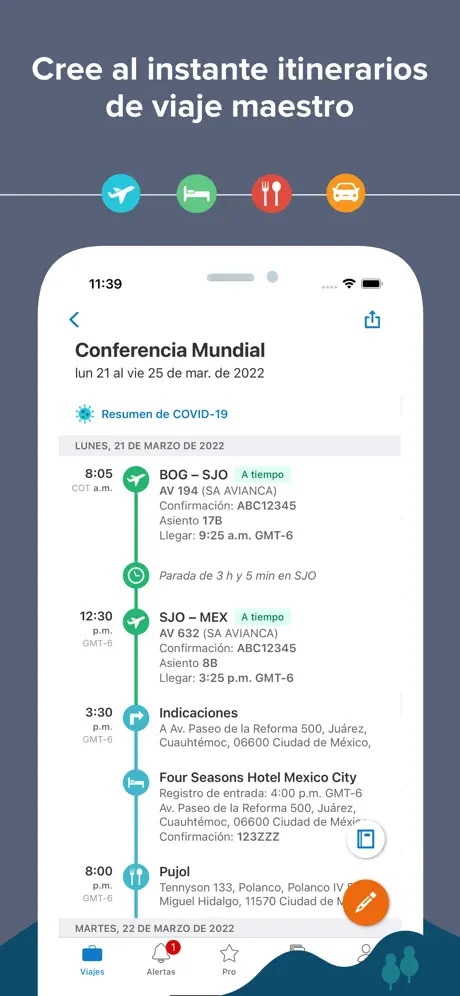
\includegraphics[width=0.20\textwidth]{images/tripit1}
    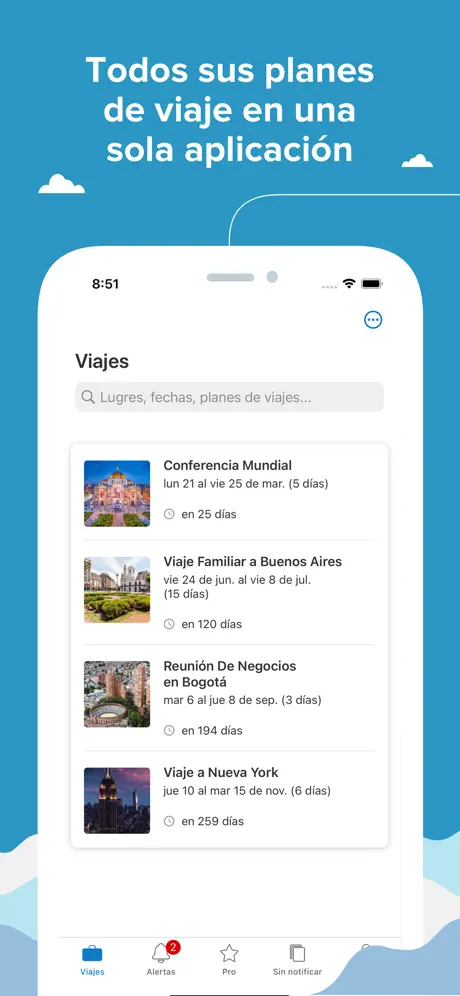
\includegraphics[width=0.20\textwidth]{images/tripit2}
    \figcaption{Capturas de pantalla de la aplicación TripIt}{\sourcelink{App Store para iPhone}{https://apps.apple.com/ar/app/tripit-travel-planner/id311035142}}%
    \label{fig:tripit}
\end{figure}

\begin{revisado}

La aplicación no solo muestra una vista de itinerario integrada en función de los distintos correos electrónicos que se
hayan reenviado sino que también permite agregar datos de eventos manualmente.
También ofrece funcionalidad para obtener direcciones a puntos de interés (como el aeropuerto o la estación de tren) y
en el caso de medios de transporte puede incluir alertas de cambio y retrasos.

Dado que es una solución comercial no se da a conocer cuáles son las técnicas que utiliza para procesar los correos
electrónicos pero consultando en la documentación oficial se puede apreciar una lista de \textit{vendors} o proveedores
de servicios de viaje que soporta la aplicación.
Se mencionan cientos de proveedores distintos en correos electrónicos escritos en inglés, español, francés, alemán y
japonés~\cite{tripit-supported-sites}.
Esta lista puede darnos un indicio de que la aplicación ha dedicado recursos para poder procesar cada uno de los correos
electrónicos de los proveedores de servicios de viajes indicando que es probable que utilice una serie de plantillas
predefinidas y un conjunto de reglas que se crean especialmente para cada proveedor.

Un punto negativo a destacar sobre esta aplicación es la privacidad, es necesario reenviar a la aplicación correos
electrónicos que contienen datos sensibles de los usuarios que son parte de la confirmación.
Por ejemplo para una reserva de un ticket de vuelo en el mail aparecerán el nombre completo del usuario, número de
pasaporte, nacionalidad, entre otros.

\end{revisado}

\FloatBarrier{}

\subsubsection{KDE Itinerary}

\begin{revisado}

En el ámbito del software libre se encuentra la aplicación~\cite{kde-itinerary-home} que consiste en una solución
enfocada en la privacidad del usuario.
Utiliza una biblioteca KItinerary, también \textit{open-source}, que provee un motor de extracción de datos de correos
electrónicos de viajes sin enviarlos a un servidor remoto.
Al igual que TripIt, esta aplicación admite reservas de distinto tipo y ofrece actualizaciones en tiempo real para
ciertos tipos de reserva.
En la \autoref{fig:kdeitinerary} se puede ver la interfaz de la versión móvil que puede descargarse desde la tienda de
aplicaciones de Android.

Luego de consultar el código fuente disponible en el repositorio oficial de~\cite{k-itinerary-repo} se pueden apreciar
actualizaciones frecuentes de la misma donde se indican cambios para soportar nuevos proveedores de servicios como así
también para mantenerse al día con las actualizaciones de las estructuras de los correos electrónicos de proveedores ya
soportados.
En cuanto a la implementación se emplea una combinación de técnicas que incluyen detección de palabras clave,
utilización de expresiones regulares para formatos comunes de fecha y hora, y ciertas heurísticas basadas en el
contenido HTML del correo.

\end{revisado}

\begin{figure}[htbp]
    \centering
    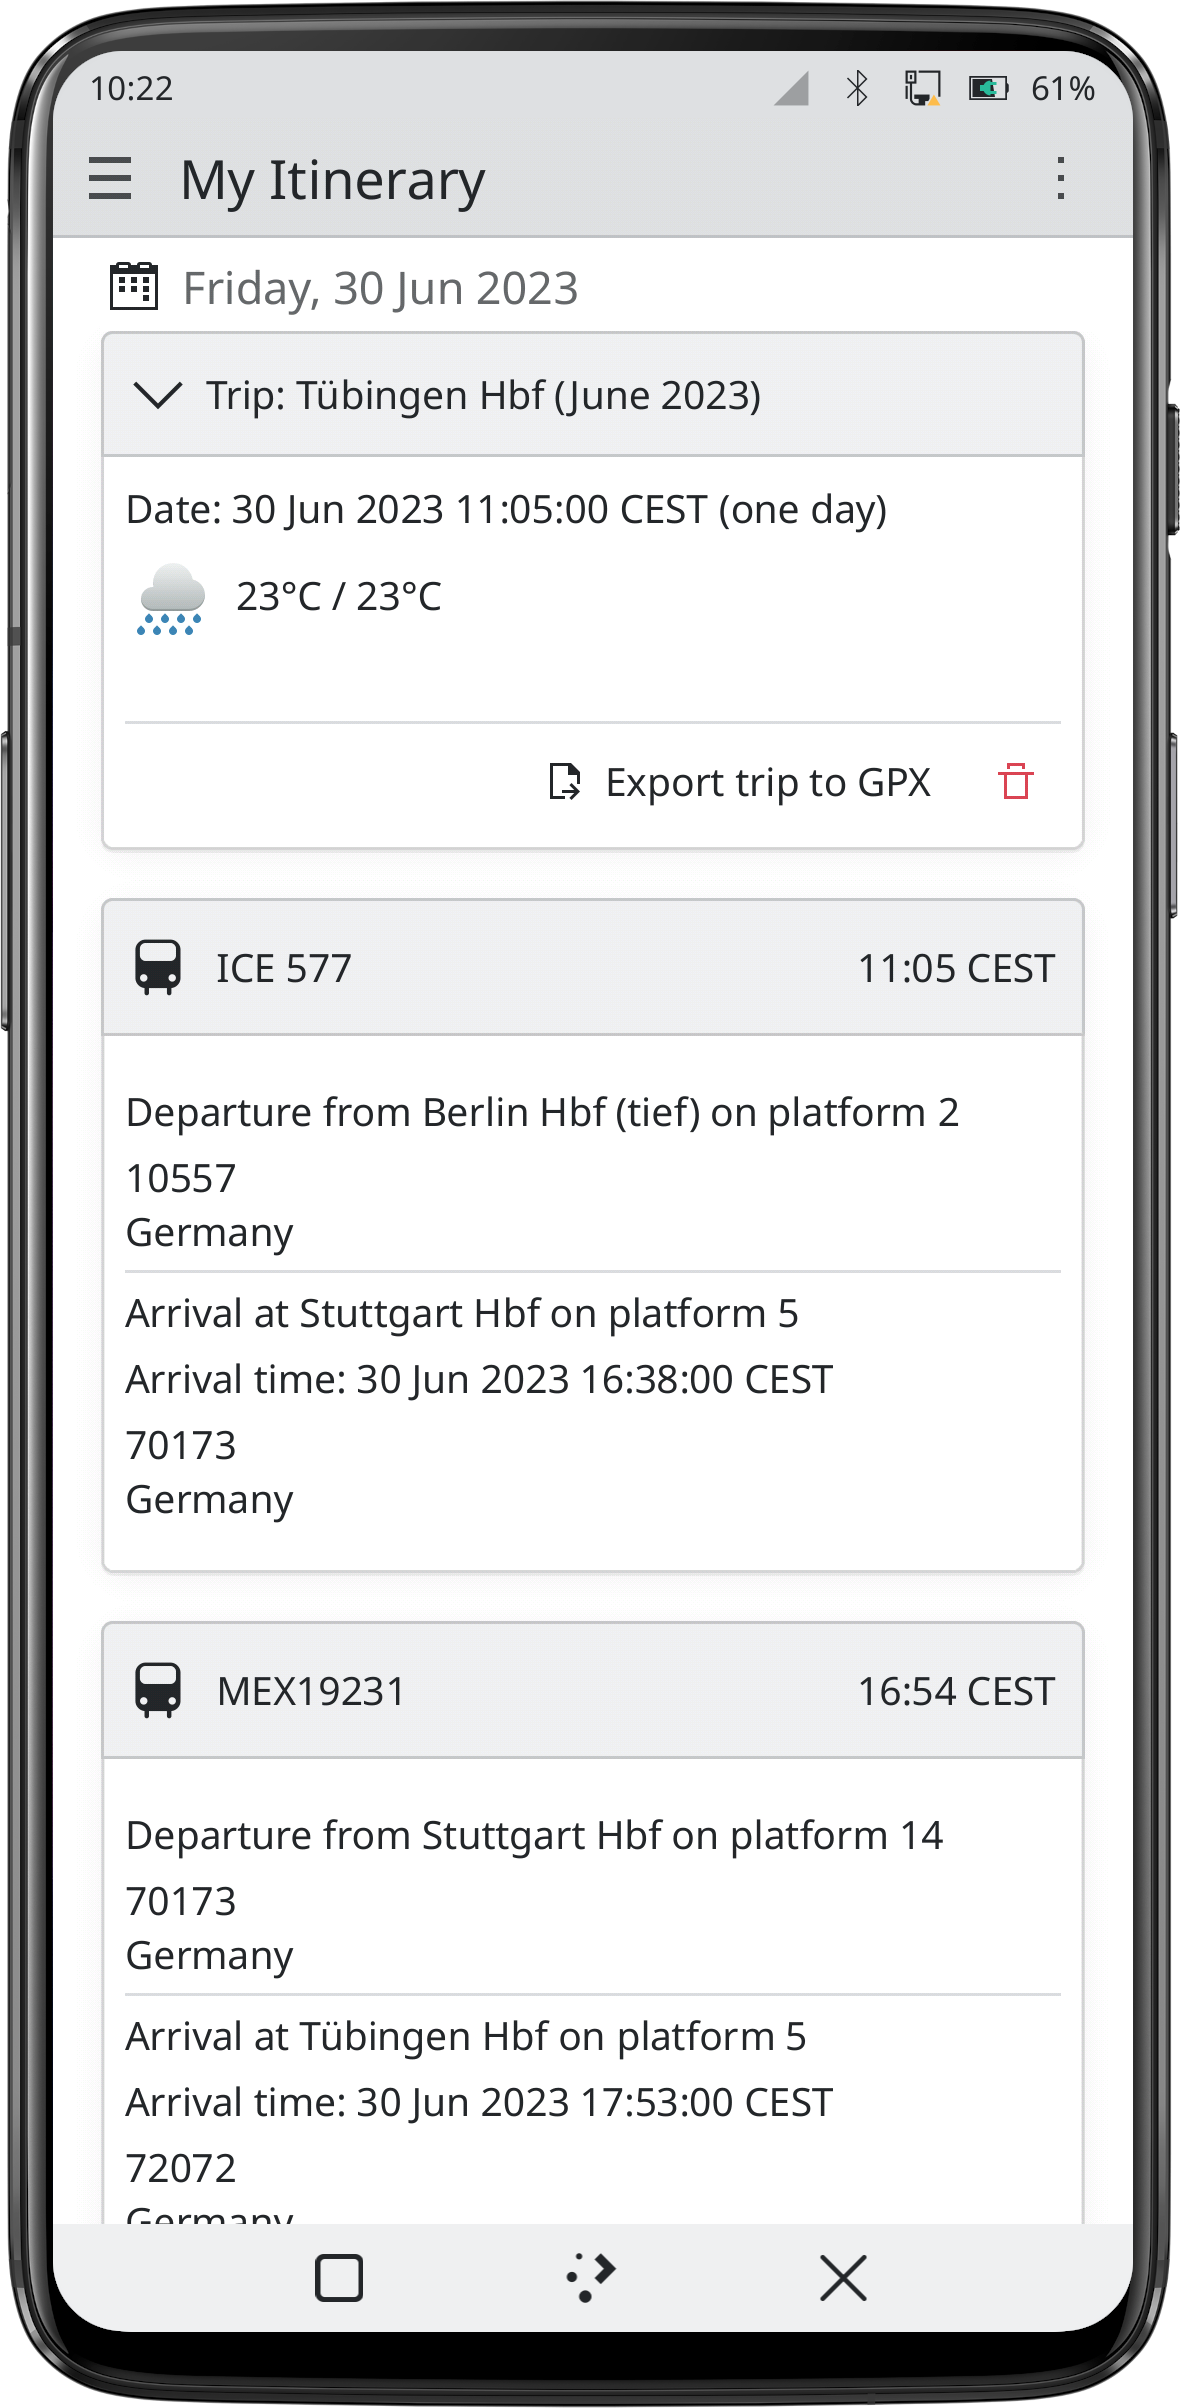
\includegraphics[width=0.20\textwidth]{images/kde1}
    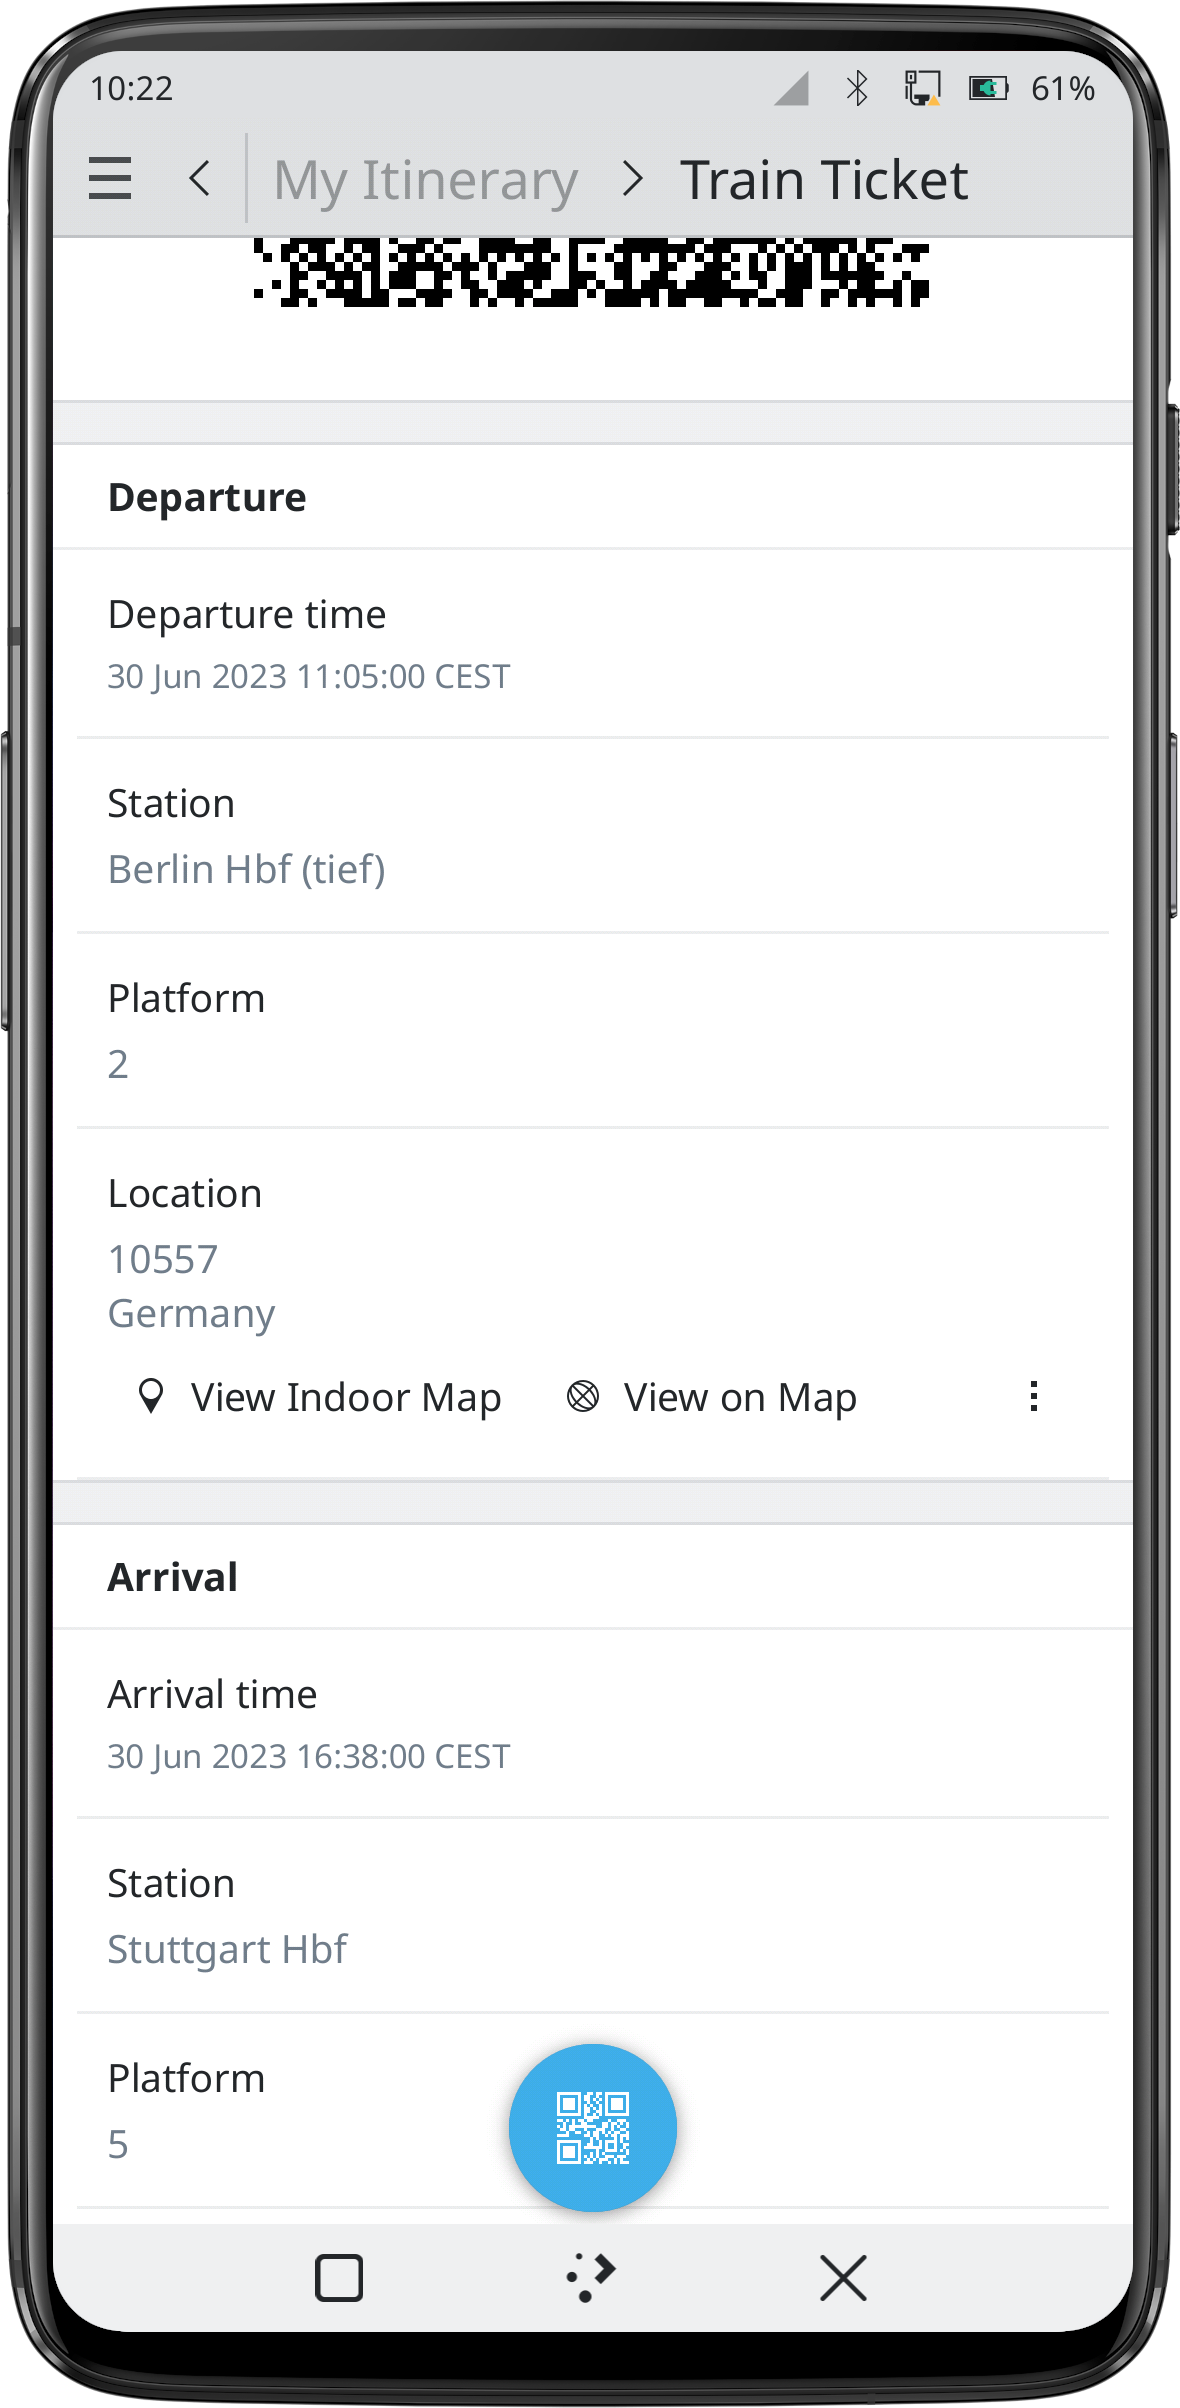
\includegraphics[width=0.20\textwidth]{images/kde2}
    \figcaption{Capturas de pantalla de la aplicación KDE Itinerary}{\sourcelink{KDE Apps}{https://apps.kde.org/es/itinerary/}}%
    \label{fig:kdeitinerary}
\end{figure}

\FloatBarrier{}

\subsubsection{Amadeus Self-Service APIs: Trip Parser}

\begin{revisado}

Por último mencionamos la función de~\cite{amadeus-trip-parser} perteneciente al servicio Self-Service APIs de Amadeus.
Amadeus IT Group es una empresa líder en el ámbito del turismo que provee soluciones tecnológicas que abarcan los
sistemas de reservas que utilizan aerolíneas, aeropuertos, proveedores de hospedaje y agencias de viajes entre otros.
Amadeus ofrece un conjunto de APIs para permitir la integración de sistemas de terceros tanto para realizar y
administrar reservas como así también ofrecer recomendaciones para futuras reservas.

El servicio Trip Parser que ofrece Amadeus consiste en un método que recibe uno o varios correos electrónicos de
reservas (codificados en el formato Base64) y extrae información de todos ellos agregándola en un único archivo JSON que
contendrá toda la información del itinerario correspondiente.
Esta solución paga para desarrolladores soporta contenido en HTML, EML y PDF de más de 300 proveedores distintos en 27
lenguajes y puede ser utilizada por cualquier aplicación web o móvil que quiera atender el problema planteado.

Cabe destacar que la API
%(Ver \autoref{fig:amadeus})
ha sido deprecada por Amadeus por lo que es probable que deje de funcionar en un futuro.

%\begin{figure}[htbp]
%    \centering
%    \includegraphics[width=0.75\textwidth]{images/amadeus1.png}
%    \caption{Sitio web de Trip Parser del portal de desarrolladores de Amadeus}
%    \label{fig:amadeus}
%\end{figure}

%\FloatBarrier{}
%\section{Hipótesis}

%Es posible generar una vista integral de la información de reservas de viaje a partir de la extracción de datos relevantes presentes en los mails de confirmación, independientemente del proveedor de servicio y de la estructura de mail utilizada.

%\subsection{Variables}

%A continuación se detalla el primer conjunto de variables a ser adoptadas para su tratamiento, clasificadas según su tipo (independiente, dependiente o contextual):

%\begin{itemize}
%\item \textbf{Datos relevantes (variable dependiente):} Para reservas de vuelos se debe extraer el nombre del pasajero, el código de reserva, la fecha y hora de salida y llegada, el aeropuerto de salida y llegada y datos del vuelo como el código y la aerolínea. En el caso de reservas de hoteles se debe extraer el nombre del hotel, la dirección, la fecha y hora de checkin y checkout.
%\item \textbf{Mails de confirmación (variable independiente)}: El contenido del mail de confirmación que contiene todos los datos relevantes en distintas formas de presentación.
%\item \textbf{Reservas de viaje (variable dependiente)}: Reservas de vuelos y reservas de hoteles.
%\item \textbf{Proveedor del Servicio (variable contextual)}: El emisor del mail de confirmación, un sitio web que realiza la reserva (por ejemplo Booking, sitios web de las aerolíneas, etc).
%\item \textbf{Estructura del mail (variable contextual)}: Como se organiza el texto del mail a analizar.
%\end{itemize}

\end{revisado}
